\begin{figure}[t]
   \centering
   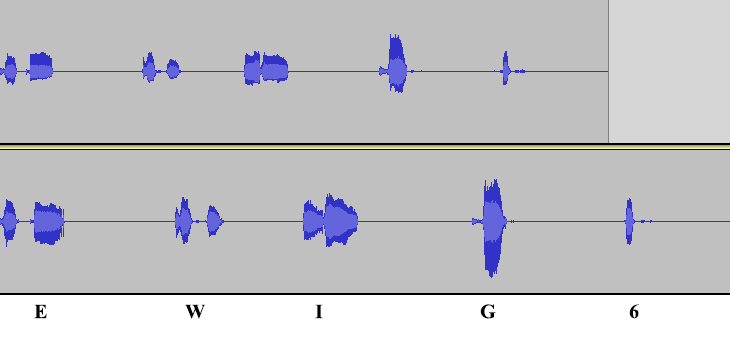
\includegraphics[width=\columnwidth]{figures/Telerik1.jpg}.
   \caption{Waveforms of Telerik's CAPTCHA, before and after processing, representing "EWIG6".}
   \label{fig:telerik1}
\end{figure}

\section{Experimental Evaluation}
\label{sec:evaluation}

This section describes the experiments we ran to evaluate our system against each CAPTCHA service. Initially, we ran a live attack with our improvised system with 50 challenges for each CAPTCHA system. We did this attack individually for all 5 solvers - IBM Watson US Accent, IBM Watson UK Accent, Wit.ai, Google Speech API US Accent and Google Speech API UK Accent. The details of the live attack are described in brief detail below.\newline

Based on the results of these experiments, we identified one solver to be the best for each CAPTCHA system. Then we did a larger attack with 1000 CAPTCHAs for each service with the identified best solver and recorded the results of whether our response got accepted or not. For each challenge we solved, we also recorded the time it took to solve that challenge. 

\begin{itemize}
\item \textbf{Apple} : To test Apple's CAPTCHAs, we launched a live attack on the Apple ID creation page. We ran our crawler on the page multiple times, filling all the text fields and dropdown boxes with random values and then downloading the audio challenge from chrome's media-internals page. The downloaded file was then sent to Audacity to get the cleaner version using the Action chain described in the previous section and the resulting .wav file was sent to the speech recognition services for transcription. After the results were obtained and entered back into the response box, if the CAPTCHA was solved properly, a 2-factor authentication dialog box was displayed. The presence of this dialog box with class \textit{step-verify-code} was checked for and the results were logged accordingly.

\item \textbf{BotDetect} : To test our system against BotDetect, we attacked the demo page of BotDetect present in \textit{www.captcha.com}. The demo page randomizes the length of the audio challenge(4-6) and the type of noise(10 noise files) added in the background so that we get a completely different kind of audio challenge each time the page is loaded. We downloaded the challenge from this demo page and solved it using our solvers after denoising. We looked for the presence of "Correct!" or "Incorrect!" in the div next to the Submit button after it is validated. 

\item \textbf{captcha.net}: captchas.net is an open-source CAPTCHA system. So we hosted this service on our test page and performed our live attack on this URL. We scraped the audio MP3 file from the loaded URL and cleaned it using Audacity and then solved it using our solvers. The resulting page either displayed "\textit{You entered the wrong password. Aren't you a human?}" or "\textit{Your message was verified to be entered by a human}". We looked for this element and then validated our solver.

\item \textbf{Microsoft Live} : The Microsoft account creation page is where we launched our attack. However, we did not perform a live attack for this one because there was no way to validate the CAPTCHA before the page was submitted. If we did submit the page, there were no further steps. A spam account would get created if the response to the CAPTCHA was right. So we decided to do an offline attack by just scraping 100 CAPTCHA challenges from Live's page and then manually listening to the audio files to get the transcription. To get a valid truth value, 3 people were asked to listen to the 100 audio files and write down their transcriptions manually. When our solvers gave us transcriptions after denoising, 

\item \textbf{reCAPTCHA V1} : The 2014 version of Google's reCAPTCHA is still available in a demo page offered by Google in the URL \textit{https://www.google.com/recapt\newline-cha/demo/}. We performed a live attack on the demo page. Once our system cleaned up the audio file and got the results back from the solvers, we looked for the presence of the text "Correct" and "Incorrect" on the top of the page.

\item \textbf{reCAPTCHA V2} : We tested our system against Google's NoCAPTCHA reCAPTCHA (Jan 2017 version) on an incognito mode. We clicked on the checkbox CAPTCHA and clicked on the Audio icon on the Image challenge iframe to get to the Audio CAPTCHA. We then downloaded the .mp3 file and solved it using our system. We looked for the presence of tick mark to verify that the challenge was solved correctly. To get past the rate limiting that Google had, we found an implementation bug in Google's reCAPTCHA that considered requests with unique user-agent strings as trust-worthy. So we generated unique user-agent strings with current timestring value.

\item \textbf{Securimage} : Securimage is again an open-source CAPTCHA system. So we hosted the service on our test page and performed our live attack on this URL. The URL when loaded dynamically constructed an audio CAPTCHA from the 26 files for 26 alphabets and the 6 noise files it had. We scraped this audio WAV file from the loaded URL and cleaned it using Audacity and then solved it using our solvers. The resulting page after submission either displayed "\textit{Incorrect security code entered}" or "\textit{The CAPTCHA was correct.}". We looked for this element and then validated our solver.

\item \textbf{Telerik} : Telerik offers a demo page for its Audio CAPTCHAs for ASP.NET developers. We performed a live attack on this page, scraping the audio files and cleaning it using Audacity using an Action Chain. The resulting WAV file was sent to the speech recognition APIs and the transcription was obtained. The presence of the text "Page submitted successfully" or "Page not valid" was checked for and recorded.
\end{itemize}